\documentclass[aspectratio=169]{beamer}
\usetheme{metropolis}
\usepackage[T1]{fontenc}
\usepackage{booktabs}
\usepackage{graphicx}
\usepackage{tabularx}
\usepackage{tikz}
\usetikzlibrary{arrows.meta,positioning,shapes.geometric}

\metroset{
  progressbar=frametitle,
  numbering=fraction,
  block=fill
}

\definecolor{ILABNavy}{HTML}{071B2F}
\definecolor{ILABBlue}{HTML}{123C69}
\definecolor{ILABOrange}{HTML}{F97316}
\definecolor{ILABGold}{HTML}{FDBA2D}
\definecolor{ILABTeal}{HTML}{13A89E}
\definecolor{ILABInk}{HTML}{142033}
\definecolor{ILABSteel}{HTML}{556270}
\definecolor{ILABLine}{HTML}{D8DEE8}
\definecolor{ILABPaper}{HTML}{F7F8FA}

\setbeamercolor{normal text}{fg=ILABInk,bg=white}
\setbeamercolor{frametitle}{fg=white,bg=ILABNavy}
\setbeamercolor{progress bar}{fg=ILABOrange,bg=ILABLine}
\setbeamercolor{alerted text}{fg=ILABOrange}
\setbeamercolor{block title}{fg=white,bg=ILABBlue}
\setbeamercolor{block body}{fg=ILABInk,bg=ILABPaper}
\setbeamercolor{title separator}{fg=ILABOrange}
\setbeamerfont{frametitle}{size=\Large,series=\bfseries}
\setbeamerfont{title}{size=\Large,series=\bfseries}
\setbeamerfont{subtitle}{size=\large}
\setbeamersize{text margin left=8mm,text margin right=8mm}

\newcommand{\code}[1]{{\ttfamily\detokenize{#1}}}
\newcommand{\pathref}[1]{{\scriptsize\ttfamily\detokenize{#1}}}
\newcommand{\smallpath}[1]{{\tiny\ttfamily\detokenize{#1}}}
\newcommand{\tightsep}{\vspace{0.35em}}
\newcommand{\ok}{\textcolor{ILABTeal}{ready}}
\newcommand{\gated}{\textcolor{ILABOrange}{operator-gated}}
\newcommand{\watch}{\textcolor{ILABGold}{watch}}
\newcommand{\chip}[1]{\begingroup\setlength{\fboxsep}{2pt}\colorbox{ILABOrange!16}{\scriptsize\textcolor{ILABNavy}{#1}}\endgroup}

\newcommand{\dotgrid}[1][ILABOrange!48]{%
  \begin{scope}[shift={(current page.north east)},x=0.18cm,y=0.18cm]
    \foreach \x in {0,...,9} {
      \foreach \y in {0,...,4} {
        \fill[#1] (-4-\x,-3-\y) circle (0.08);
      }
    }
  \end{scope}
}

\newcommand{\sectionframe}[2]{%
  \begin{frame}[plain]
    \begin{tikzpicture}[remember picture,overlay]
      \fill[ILABNavy] (current page.south west) rectangle (current page.north east);
      \fill[ILABOrange] (current page.south west) rectangle ([xshift=0.34cm]current page.north west);
      \draw[ILABOrange,line width=1.2pt] ([xshift=1.1cm,yshift=-1.55cm]current page.north west) -- ++(4.3cm,0);
      \dotgrid[ILABOrange!55]
    \end{tikzpicture}
    \vspace*{1.15cm}
    {\color{ILABOrange}\Large #1\par}
    \vspace{0.55cm}
    {\color{white}\Large\bfseries #2\par}
  \end{frame}
}

\newcommand{\decktitleframe}[4]{%
  \begin{frame}[plain]
    \begin{tikzpicture}[remember picture,overlay]
      \fill[ILABNavy] (current page.south west) rectangle (current page.north east);
      \fill[ILABOrange] (current page.south west) rectangle ([xshift=0.36cm]current page.north west);
      \node[anchor=east,opacity=0.33] at ([xshift=-0.55cm,yshift=-0.25cm]current page.east) {
        \includegraphics[height=0.88\paperheight]{#4}
      };
      \dotgrid[ILABOrange!62]
    \end{tikzpicture}
    \vspace*{0.95cm}
    {\color{ILABOrange}\Large #1\par}
    \vspace{0.35cm}
    {\color{white}\Large\bfseries #2\par}
    \vspace{0.35cm}
    {\color{white!78}\large\parbox{0.58\paperwidth}{#3}\par}
    \vfill
    {\color{white!72}\normalsize pctiope/smart-i-lab-testbed \hfill May 2026\par}
  \end{frame}
}

\tikzset{
  ilabbox/.style={
    draw=ILABLine,
    fill=white,
    rounded corners=2pt,
    align=center,
    minimum height=0.82cm,
    font=\scriptsize
  },
  ilabdark/.style={
    draw=white!28,
    fill=white!7,
    rounded corners=2pt,
    align=center,
    minimum height=0.82cm,
    font=\scriptsize,
    text=white
  },
  ilabstore/.style={
    draw=ILABTeal,
    cylinder,
    shape border rotate=90,
    aspect=0.22,
    fill=ILABTeal!12,
    align=center,
    font=\scriptsize,
    minimum height=1.0cm
  },
  ilabflow/.style={-Latex,draw=ILABOrange,line width=1.1pt},
  ilabthinflow/.style={-Latex,draw=ILABSteel,line width=0.9pt},
  ilablane/.style={draw=ILABLine,fill=ILABPaper,rounded corners=3pt}
}


\title{Smart i-LAB AIR1 All-Zones}
\subtitle{Applied research overview for room-level all-zones occupancy estimation}
\author{pctiope/smart-i-lab-testbed}
\date{May 2026}

\begin{document}

\decktitleframe{Applied Research Overview}{Smart i-LAB AIR1 All-Zones}{Room-level occupancy estimation from two cameras and shared environmental sensing}{../../../Smart-iLab_DigitalTwin/assets/smart_ilab_3d/Smart_I-LAB_floor3d_room_8_44.jpg}

\begin{frame}[shrink=6]{Problem Motivation}
\begin{columns}[T,onlytextwidth]
\column{0.49\textwidth}
\begin{tikzpicture}
  \node[anchor=west] at (0,0) {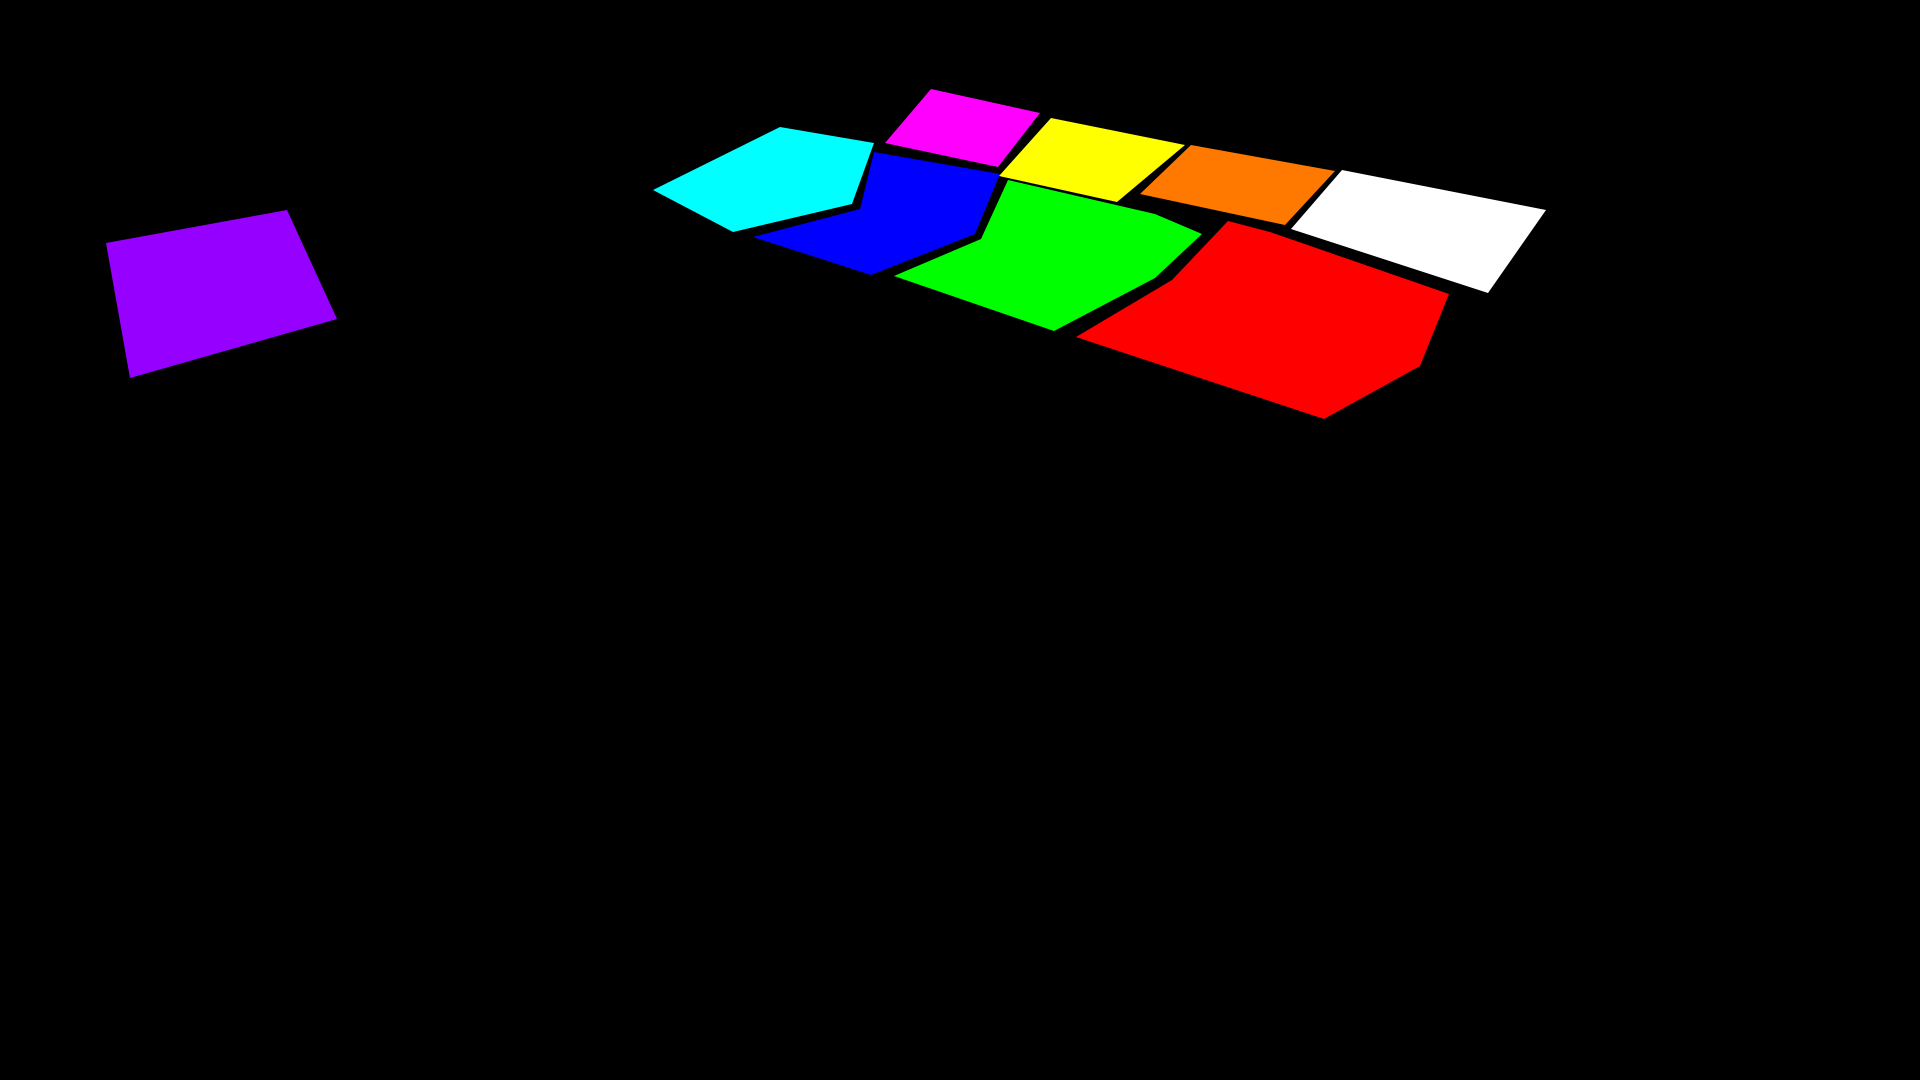
\includegraphics[width=0.94\linewidth,height=0.24\textheight,keepaspectratio]{../../../air1_all_zones_cv_time_features_package/masks/cam1-mask-zones.png}};
  \node[anchor=west] at (0,-1.70) {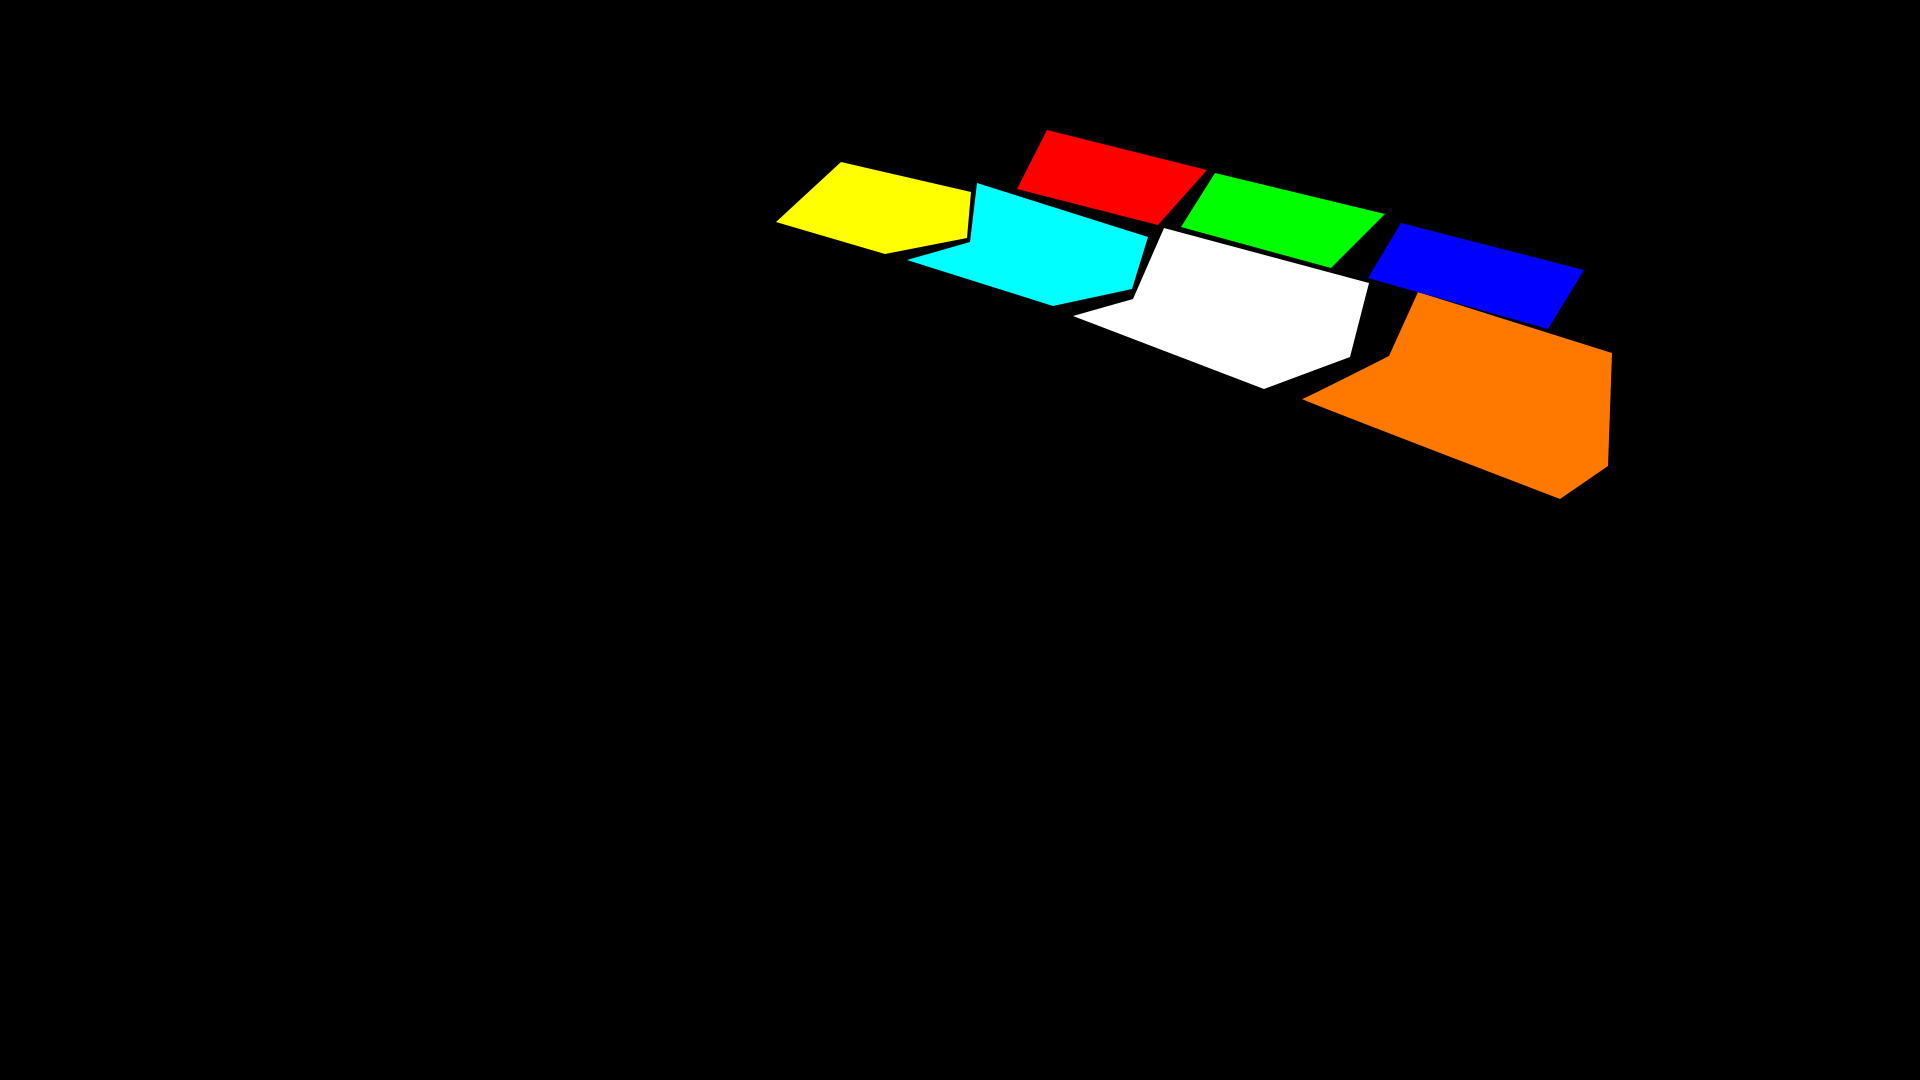
\includegraphics[width=0.94\linewidth,height=0.24\textheight,keepaspectratio]{../../../air1_all_zones_cv_time_features_package/masks/cam2-mask-zones.png}};
  \node[anchor=south west,fill=ILABNavy,text=white,inner sep=2pt,font=\tiny] at (0.1,0.72) {cam1 zones};
  \node[anchor=south west,fill=ILABNavy,text=white,inner sep=2pt,font=\tiny] at (0.1,-0.98) {cam2 zones};
\end{tikzpicture}
\vspace{0.2em}

{\tiny\textcolor{ILABSteel}{Tracked camera-zone masks define AIR1 coverage.}\par}

\column{0.47\textwidth}
\begin{block}{Research setting}
AIR1 asks for room-level occupancy over zones 1--15. The evidence is not one
desk, one camera, or one sensor stream: two camera views, per-zone masks, shared
AIR-1 readings, SEN55 readings, and readiness gates all shape the result.
\end{block}
\tightsep
\begin{itemize}
  \item Camera coverage differs by zone and can be missing for a timestamp.
  \item The dashboard should remain useful before a production model is promoted.
  \item The model must not borrow Zone 5 power or mmWave assumptions.
\end{itemize}
\end{columns}
\end{frame}

\begin{frame}[shrink=3]{Research Gap}
\begin{columns}[T,onlytextwidth]
\column{0.48\textwidth}
\textbf{What all-zones changes}
\begin{itemize}
  \item A room model must preserve per-zone labels, not collapse the room into one binary stream.
  \item Long-form \code{timestamp + zone_id} rows need split, grouping, audit, and display discipline.
  \item Missing camera coverage should remain unknown, not become vacancy.
\end{itemize}

\column{0.48\textwidth}
\begin{block}{Gap addressed here}
\small
AIR1 is framed as an all-zones applied-research pipeline: per-zone CV labels,
two-camera coverage, shared environmental features, null-preserving labels, and
model-readiness gates are evaluated together.
\end{block}
\tightsep
\chip{Zones 1--15}
\hspace{0.35em}
\chip{Two cameras}
\hspace{0.35em}
\chip{No power/mmWave}
\end{columns}
\end{frame}

\begin{frame}{Research Questions}
\begin{enumerate}
  \item Can one shared model represent zones 1--15 from long-form \code{timestamp + zone_id} rows?
  \item Can per-zone CV labels stay null when coverage is missing instead of becoming false negatives?
  \item Can the AIR1 dashboard stay useful while inference is gated by production model readiness?
\end{enumerate}
\tightsep
\begin{center}
\parbox{0.84\textwidth}{\centering
\small The AIR1 deck keeps Zone 5-specific power, mmWave, and CI/CD scope out of the model narrative except as contrast.}
\end{center}
\end{frame}

\begin{frame}[shrink=4]{System And Method Overview}
\begin{columns}[T,onlytextwidth]
\column{0.48\textwidth}
\textbf{Method}
\begin{itemize}
  \item Use cam1 and cam2 masks to emit per-zone CV counts.
  \item Aggregate labels into 10-second \code{timestamp + zone_id} buckets.
  \item Join AIR-1 and SEN55 features into long-form rows for model zones 1--15.
  \item Use \code{occupied} as the target and keep \code{zone_id} for grouping, audits, splits, and display.
  \item Gate live inference on a promoted production pointer while keeping camera/dashboard health visible.
\end{itemize}

\column{0.48\textwidth}
\centering
\resizebox{0.98\linewidth}{!}{%
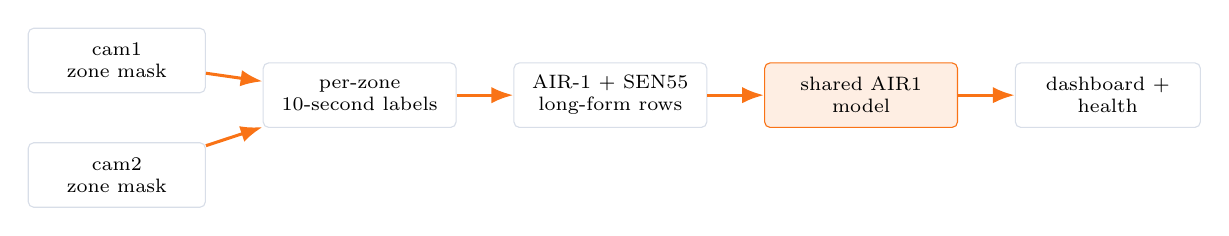
\begin{tikzpicture}[node distance=0.62cm and 0.72cm]
  \node[ilabbox,minimum width=2.25cm] (cam1) {cam1\\zone mask};
  \node[ilabbox,below=of cam1,minimum width=2.25cm] (cam2) {cam2\\zone mask};
  \node[ilabbox,right=of cam1,yshift=-0.44cm,minimum width=2.45cm] (labels) {per-zone\\10-second labels};
  \node[ilabbox,right=of labels,minimum width=2.45cm] (features) {AIR-1 + SEN55\\long-form rows};
  \node[ilabbox,right=of features,minimum width=2.45cm,fill=ILABOrange!12,draw=ILABOrange] (model) {shared AIR1\\model};
  \node[ilabbox,right=of model,minimum width=2.35cm] (app) {dashboard +\\health};
  \draw[ilabflow] (cam1) -- (labels);
  \draw[ilabflow] (cam2) -- (labels);
  \draw[ilabflow] (labels) -- (features);
  \draw[ilabflow] (features) -- (model);
  \draw[ilabflow] (model) -- (app);
\end{tikzpicture}
}
\tightsep
\begin{block}{Contract boundary}
\small AIR1 model inputs are AIR-1, SEN55, missing indicators, and time features. Power, mmWave, and \code{zone_id} are excluded from the feature input.
\end{block}
\end{columns}
\end{frame}

\begin{frame}[shrink=2]{Technical Architecture As Method Evidence}
\centering
\resizebox{0.98\textwidth}{!}{%
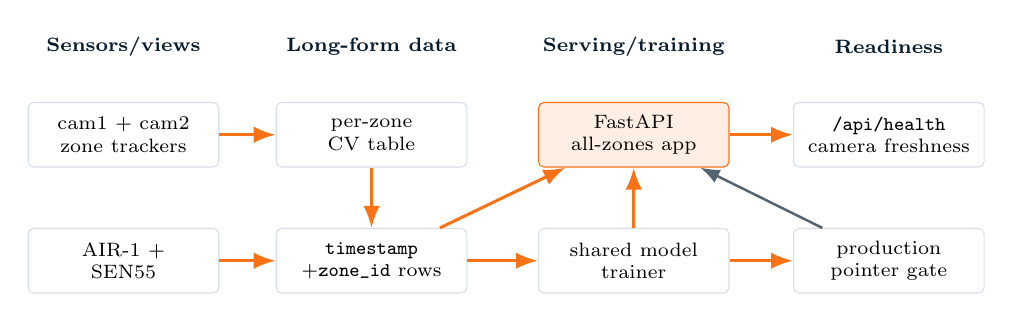
\begin{tikzpicture}[
  node distance=0.70cm and 0.82cm,
  laneTitle/.style={font=\bfseries\scriptsize,text=ILABNavy},
  box/.style={ilabbox,minimum width=2.42cm}
]
  \node[laneTitle] at (0,2.0) {Sensors/views};
  \node[laneTitle] at (3.15,2.0) {Long-form data};
  \node[laneTitle] at (6.48,2.0) {Serving/training};
  \node[laneTitle] at (9.72,2.0) {Readiness};

  \node[box] (views) at (0,0.88) {cam1 + cam2\\zone trackers};
  \node[box] (env) at (0,-0.72) {AIR-1 +\\SEN55};
  \node[box] (labels) at (3.15,0.88) {per-zone\\CV table};
  \node[box] (rows) at (3.15,-0.72) {\code{timestamp}\\+\code{zone_id} rows};
  \node[box,fill=ILABOrange!12,draw=ILABOrange] (app) at (6.48,0.88) {FastAPI\\all-zones app};
  \node[box] (trainer) at (6.48,-0.72) {shared model\\trainer};
  \node[box] (health) at (9.72,0.88) {\code{/api/health}\\camera freshness};
  \node[box] (pointer) at (9.72,-0.72) {production\\pointer gate};

  \draw[ilabflow] (views) -- (labels);
  \draw[ilabflow] (env) -- (rows);
  \draw[ilabflow] (labels) -- (rows);
  \draw[ilabflow] (rows) -- (app);
  \draw[ilabflow] (rows) -- (trainer);
  \draw[ilabflow] (trainer) -- (app);
  \draw[ilabflow] (app) -- (health);
  \draw[ilabflow] (trainer) -- (pointer);
  \draw[ilabthinflow] (pointer) -- (app);
\end{tikzpicture}
}
\tightsep
\begin{center}
\chip{Null-preserving labels}
\hspace{0.45em}
\chip{Shared model}
\hspace{0.45em}
\chip{Per-zone dashboard}
\hspace{0.45em}
\chip{Readiness before inference}
\end{center}
\end{frame}

\begin{frame}[shrink=4]{Labeling And Feature Contract}
\begin{columns}[T,onlytextwidth]
\column{0.48\textwidth}
\textbf{Label contract}
\begin{itemize}
  \item Target: \code{occupied}.
  \item Key: one row per \code{timestamp + zone_id}.
  \item Positive rule: per-zone median \code{occupancy_count >= 1}.
  \item No matching CV label means \code{occupied = null}.
  \item Table 16 is visible camera context but excluded from model zones.
\end{itemize}

\column{0.48\textwidth}
\textbf{Feature contract}
\begin{itemize}
  \item Valid model zones are 1--15.
  \item Inputs: AIR-1 environment, SEN55 fields, missing indicators, and time cycles.
  \item \code{zone_id} supports grouping, windows, audits, splits, and display only.
  \item No power or mmWave features are imported from Zone 5.
\end{itemize}
\end{columns}
\end{frame}

\begin{frame}[shrink=3]{Evaluation Design And Validation Gates}
\begin{columns}[T,onlytextwidth]
\column{0.48\textwidth}
\textbf{Offline validation}
\begin{itemize}
  \item Per-zone label coverage and both-class window checks.
  \item Rolling-calendar splits with hidden blind-test evidence.
  \item Contract tests for feature columns, masks, labels, and runtime payloads.
  \item Smoke checks reject wrong target columns and incompatible artifacts.
\end{itemize}

\column{0.48\textwidth}
\textbf{Runtime validation}
\begin{itemize}
  \item \code{/api/health} reports readiness, history size, camera statuses, and latest errors.
  \item Camera freshness remains visible even when inference waits for a production pointer.
  \item Missing production readiness is a gated state, not a dashboard outage.
  \item Null label coverage is audited instead of converted to vacancy.
\end{itemize}
\end{columns}
\end{frame}

\begin{frame}[shrink=4]{Dashboard Usefulness While Inference Is Gated}
\begin{columns}[T,onlytextwidth]
\column{0.48\textwidth}
\textbf{Useful before promotion}
\begin{itemize}
  \item Two MJPEG feeds can show whether cam1 and cam2 are fresh.
  \item Per-zone CV truth can be displayed independently from model probability.
  \item The health payload explains readiness blockers such as a missing production pointer.
\end{itemize}

\column{0.48\textwidth}
\begin{block}{Applied-research implication}
\small
AIR1 separates observation quality from model readiness. A dashboard can support
data collection and diagnosis before the first promotable all-zones model
exists, as long as it does not present missing inference as validated occupancy.
\end{block}
\tightsep
\chip{Collect}
\hspace{0.35em}
\chip{Audit}
\hspace{0.35em}
\chip{Gate}
\hspace{0.35em}
\chip{Promote}
\end{columns}
\end{frame}

\begin{frame}[shrink=4]{Limitations And Threats To Validity}
\begin{columns}[T,onlytextwidth]
\column{0.49\textwidth}
\textbf{Data and label threats}
\begin{itemize}
  \item Camera occlusion and zone-mask coverage can vary by table and view.
  \item Missing camera coverage creates null labels and reduces usable validation evidence.
  \item Table 16 exclusion limits model scope to zones 1--15.
  \item Calendar-window maturity can block strict rolling validation.
\end{itemize}

\column{0.47\textwidth}
\textbf{Operational threats}
\begin{itemize}
  \item Production pointer absence means inference is not ready, even if collection is alive.
  \item Sensor/API availability can affect environmental feature freshness.
  \item Training quality depends on enough occupied and unoccupied windows per split.
  \item This deck intentionally excludes Zone 5 deployment claims from AIR1 scope.
\end{itemize}
\end{columns}
\end{frame}

\begin{frame}[shrink=4]{Research Roadmap And Source Anchors}
\begin{columns}[T,onlytextwidth]
\column{0.42\textwidth}
\textbf{Roadmap}
\begin{itemize}
  \item Mature per-zone label coverage before treating all-zones inference as production-ready.
  \item Promote only after strict-window evidence, smoke checks, and contract tests pass.
  \item Keep camera freshness, null label rates, and production pointer state visible in operations.
\end{itemize}

\column{0.54\textwidth}
\tiny
\renewcommand{\arraystretch}{0.96}
\begin{tabularx}{\textwidth}{@{}lX@{}}
\toprule
\textbf{Topic} & \textbf{Primary source paths} \\
\midrule
Pipeline contract & \pathref{air1/.../PIPELINE.md} \\
Feature columns & \pathref{air1/.../feature_contract.py} \\
CV labels and masks & \pathref{air1/.../rtsp_zone_tracker.py}, \pathref{air1/.../masks/} \\
Training/promotion & \pathref{air1/.../retrain_once.py}, \pathref{air1/.../promote_model.py} \\
Runtime readiness & \pathref{air1/.../web_app/}, \pathref{air1/.../tests/} \\
\bottomrule
\end{tabularx}
\renewcommand{\arraystretch}{1.0}
\end{columns}
\tightsep
\begin{center}
\parbox{0.82\textwidth}{\centering\textbf{Closing point: AIR1 is an all-zones, two-camera occupancy study whose null labels and readiness gates are part of the method.}}
\end{center}
\end{frame}

\end{document}
